\documentclass[a4paper,12pt,twocolumn]{article}
\usepackage{tabularx} % extra features for tabular environment
\usepackage{amsmath}  % improve math presentation
\usepackage{graphicx} % takes care of graphic including machinery
\usepackage[margin=1in,letterpaper]{geometry} % decreases margins
\usepackage{cite} % takes care of citations
\usepackage[final]{hyperref} % adds hyper links inside the generated pdf file
\usepackage{booktabs,caption}
\usepackage{threeparttable}
\usepackage{graphicx} 
\usepackage{float}
\hypersetup{
	colorlinks=true,       % false: boxed links; true: colored links
	linkcolor=black,        % color of internal links
	citecolor=black,        % color of links to bibliography
	filecolor=magenta,     % color of file links
	urlcolor=black         
}

\begin{document}

\begin{titlepage}
	\begin{center}
		
		\thispagestyle{empty}
		
		\Huge{
			\textbf{UCD School Of Physics}
		}
		
		\vspace{1cm}	
		
		
\includegraphics[scale=0.08]{UCDLogo.png}
		
		\vspace{1cm}
		
		\large{
			\textbf{PHYC30170 Physics with Astronomy and Space Science Lab 1; \\
				Frequency Dependence of the Skin Depth in a Metal Cylinder \\
				\vspace{1cm}
				22/09/2022 \\
				\vspace{1cm}
				Daragh Hollman}
		} \\
		
	\end{center}
\end{titlepage}

\twocolumn[
\begin{@twocolumnfalse}
	\begin{abstract}
		The aim of this experiment was to investigate the frequency dependence of the skin effect in varying metal cylindrical conductors, and measure their conductivity. This was accomplished by measuring the induced voltage in a pick-up coil wrapped on each cylinder.
	\end{abstract}
\end{@twocolumnfalse}
]

\section{Introduction}
	In this experiment
	
\section{Theory}
	The skin effect

	Present key equations without deriving.
	
\section{Methodology}
	
	\begin{figure}
		\centering
		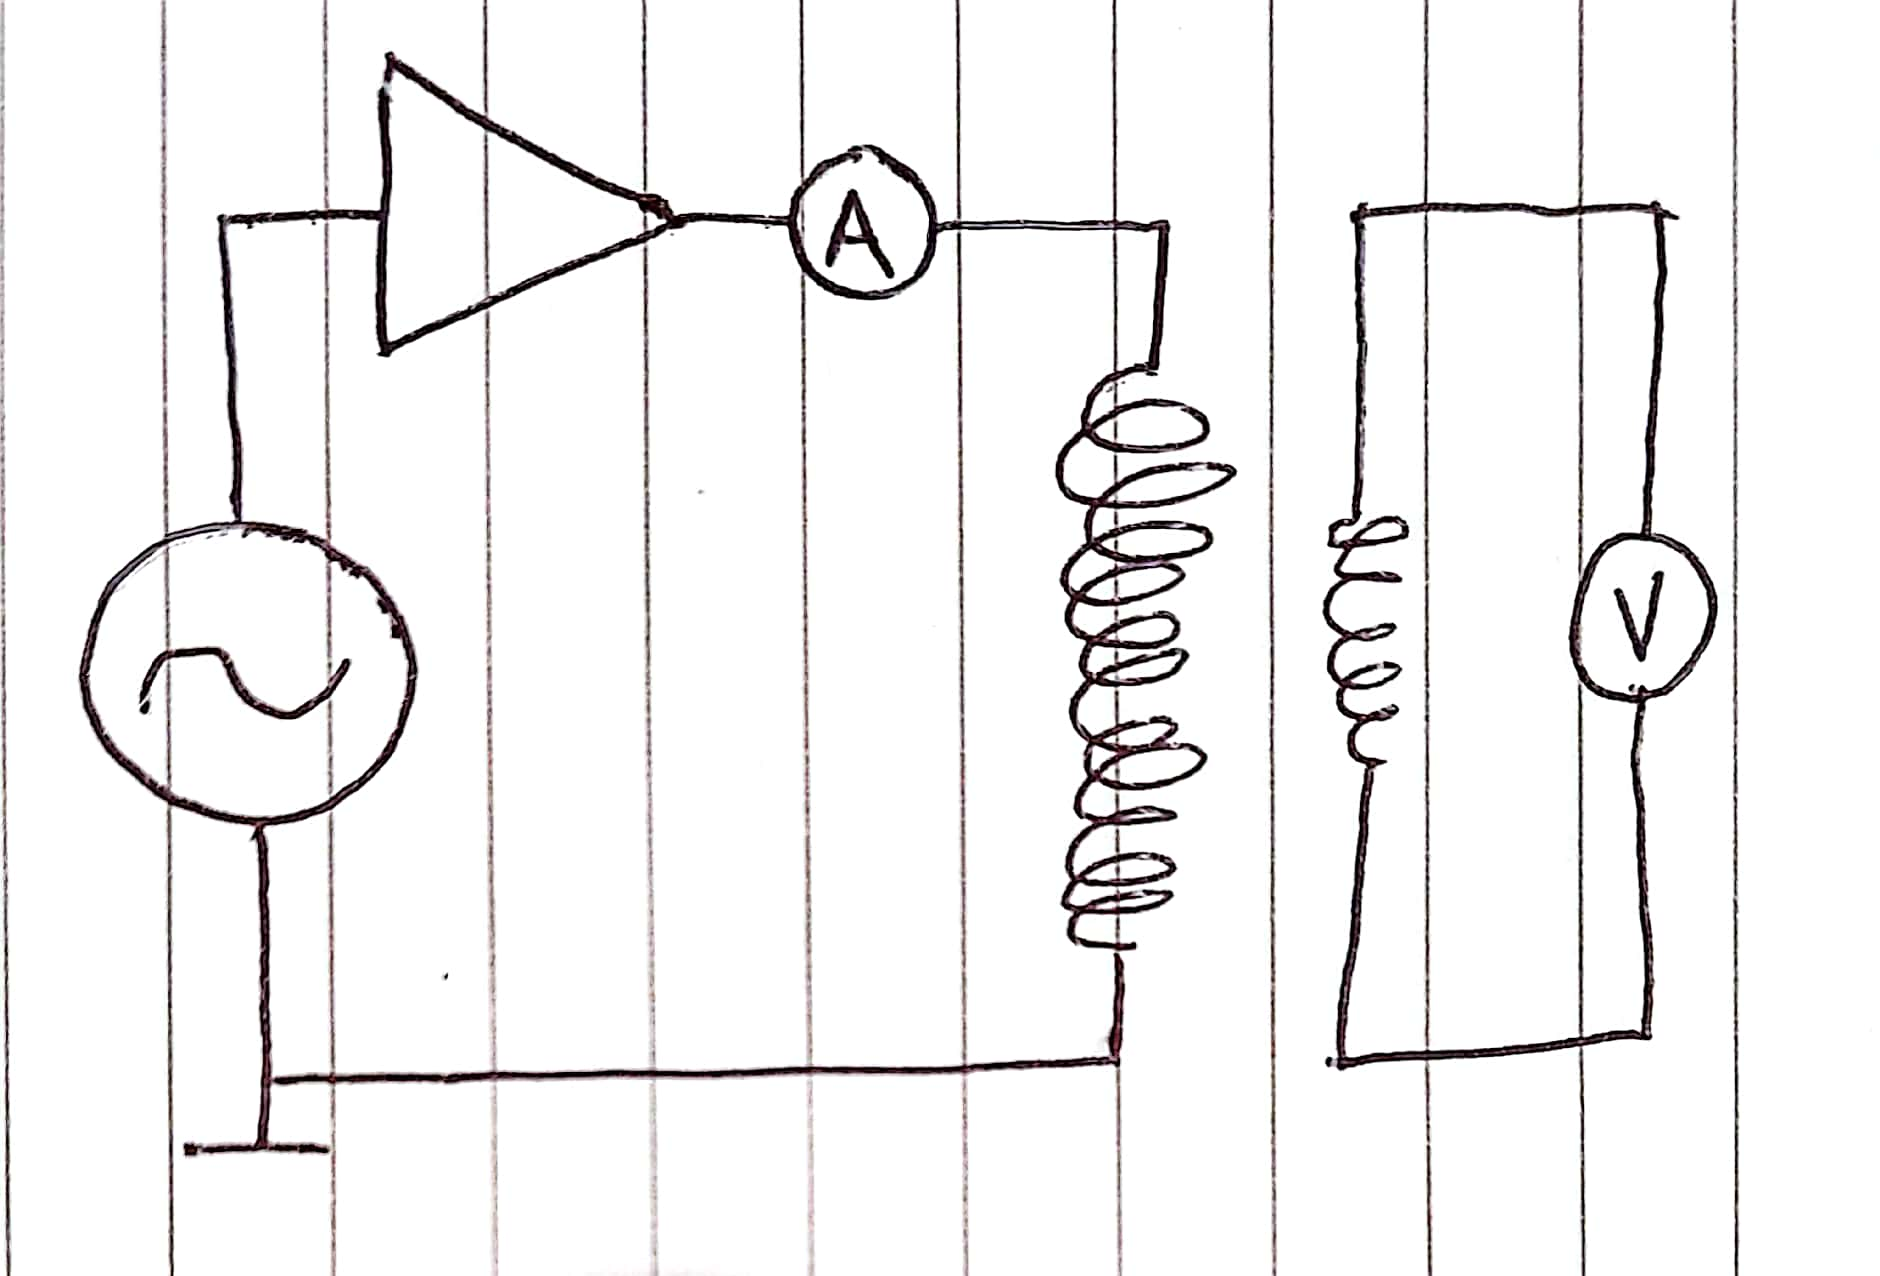
\includegraphics[scale=0.1]{SDcircuit.jpg}
		\captionsetup{font=scriptsize}
		\caption{Circuit diagram of the skin depth apparatus}
		\label{fig:circuit}
	\end{figure}

	\begin{figure}
		\centering
		\includegraphics[scale=0.045]{SDPhoto.jpg}
		\captionsetup{font=scriptsize}
		\caption{Photo of the skin depth apparatus, the metal cylinders were held inside the primary coil and  }
		\label{fig:photo}
	\end{figure}

	The apparatus was setup as shown in figures \ref{fig:circuit} and \ref{fig:photo}. The induction field was created by a solenoid of length $L_1 = (389 \pm 0.5) \,\text{mm}$ which contained $N_1 = 900 \pm $ turns of an insulated copper wire wound on a hollow tube - which the metal cylinders were inserted into. The signal to this solenoid was created by an AC signal generator and amplified. The rms current was kept constant at $I = (19 \pm 0.1)\,\text{mA}$. Although the accuracy of the ammeter used was higher, a larger uncertainty was used in practice to account for the very high sensitivity of adjusting the amplitude of the signal generator's output.
	
\section{Results and Analysis}
	Relative mu
	
	

\section{Conclusion}
	Vestibulum non facilisis sem. Quisque gravida accumsan nunc tincidunt molestie. Donec pharetra urna ut nunc ullamcorper, in tincidunt sem dignissim. Ut mattis leo eu erat elementum, id fermentum tortor sollicitudin. Vestibulum id erat in mauris aliquam vulputate non id augue. Mauris tincidunt ornare imperdiet. Aliquam tristique bibendum metus, dignissim pharetra lorem lacinia nec. Class aptent taciti sociosqu ad litora torquent per conubia nostra, per inceptos himenaeos. Maecenas sit amet pharetra leo. Morbi id hendrerit nulla. Nunc sit amet ligula risus. Mauris sed odio egestas, luctus odio at, ultricies tortor. Pellentesque semper enim vitae malesuada tempor. Aliquam at risus nisl. Curabitur venenatis, est eget hendrerit iaculis, nulla leo aliquam est, at commodo tellus arcu non eros. Nullam quis ipsum non urna porta sollicitudin.

\newpage
\begin{thebibliography}{}
	
	
\end{thebibliography}

	

\newpage

\section*{Appendices}
	
	
\end{document}
